\documentclass{amsart}
\usepackage{amsmath,amssymb,stmaryrd,pxfonts,lmodern,tikz}
\usetikzlibrary{external}

\newtheorem{prop}{Proposition}

\newcommand{\id}{\mathrm{id}}
\newcommand{\op}{\mathrm{op}}
\newcommand{\Ob}{\operatorname{Ob}}
\newcommand{\Arr}{\operatorname{Arr}}
\newcommand{\prof}{\multimapdotbothA}
\newcommand{\backref}{\vcenter{\hbox{\larger[2]$\star$}}}
\newcommand{\place}{-}
\newcommand{\base}{\mathrm{base}}
\newcommand{\transformto}{\to}
\newcommand{\canoniso}{=}
\newcommand{\posof}{\in}
\newcommand{\sub}{\mathrel{\triangleleft}}
\newcommand{\subd}{\mathrel{\!\vcenter{\hbox{\larger[-12]$\blacktriangleleft$}}\!}}
\newcommand{\idsub}{\id_{\sub}}
\newcommand{\idsubd}{\id_{\subd}}

\newcommand{\cat}[1]{\mathcal{#1}}
\newcommand{\bundle}[1]{\overset{#1}{\to}}
\newcommand{\shrink}[2][.65]{\scalebox{#1}{$#2$}}
\newcommand{\pos}[1]{#1(1)}
\newcommand{\dir}[2]{#1[#2]}
\newcommand{\posmap}[2]{{#1}_1(#2)}
% \newcommand{\dirmap}[3]{{#1}^\sharp(#2,#3)}
\newcommand{\dirmap}[3]{{#1}^\sharp_{#2}(#3)}
% \newcommand{\anydirmap}[2]{\dirmap{#1}{\place}{#2}}
\newcommand{\anydirmap}[2]{{#1}^\sharp(#2)}

\newcommand{\catname}[1]{{\normalfont\mathbf{#1}}}
\newcommand{\Set}{\catname{Set}}


\definecolor{rcol}{RGB}{255,0,0}
\definecolor{gcol}{RGB}{0,150,0}
\definecolor{pcol}{RGB}{170,0,170}
\definecolor{bcol}{RGB}{0,0,255}
\definecolor{ycol}{RGB}{210,130,0}

\tikzset{every picture/.style={scale=.1,baseline}}

\tikzset{vertex/.style={circle,draw,inner sep=1pt,minimum size=6,text=black}}
\tikzset{edge/.style={-stealth}}
\tikzset{label/.style={rectangle,rounded corners,fill=white,inner
sep=1pt,text=black}}

\tikzset{annot/.style={font=\scriptsize}}
\tikzset{dash/.style={dashed,draw opacity=0.5}}
\tikzset{transparent/.style={draw opacity=0.3,fill opacity=0.3}}
\tikzset{small/.style={minimum size=3.5}}
\tikzset{large/.style={minimum size=12}}
\tikzset{huge/.style={minimum size=17}}
\tikzset{huger/.style={minimum size=27}}
\title{Polynomial bicomodules are parametric right adjoints}
\begin{document}
\maketitle

Recall that the substitution product of polynomials $p$ and $q$,
denoted $p \sub q$, is characterized as follows.
\begin{itemize}
\item A position $a$ in $p \sub q$ consists of a position $a_\base$ in
  $p$ and positions $a_f$ in $q$ for each direction $f$ from
  $a_\base$.
\item A direction from position $a$ in $p \sub q$ consists of a
  direction $f$ from $a_\base$ and a direction $g$ from $a_f$.
\end{itemize}
\vspace{.5em}
\begin{center}
  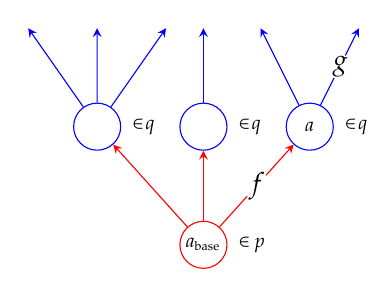
\begin{tikzpicture}
    \node [rcol,vertex,huge] (s) at (0, -12) {\scriptsize$a_{\shrink{\base}}$};
    \node [bcol,vertex,huge] (m1) at (-13.5,3) {};
    \node [bcol,vertex,huge] (m2) at (0,3) {};
    \node [bcol,vertex,huge] (m3) at (13.5,3) {\scriptsize$a$};
    \coordinate (t11) at (-22.25,15.5) {};
    \coordinate (t12) at (-13.5,15.5) {};
    \coordinate (t13) at (-4.75,15.5) {};
    \coordinate (t21) at (0,15.5) {};
    \coordinate (t31) at (7.25,15.5) {};
    \coordinate (t32) at (19.75,15.5) {};
    \draw [rcol,edge] (s) -- (m1);
    \draw [rcol,edge] (s) -- (m2);
    \draw [rcol,edge] (s) -- node [label] {$f$} (m3);
    \draw [bcol,edge] (m1) -- (t11);
    \draw [bcol,edge] (m1) -- (t12);
    \draw [bcol,edge] (m1) -- (t13);
    \draw [bcol,edge] (m2) -- (t21);
    \draw [bcol,edge] (m3) -- (t31);
    \draw [bcol,edge] (m3) -- node [label] {$g$} (t32);
    
    \node [annot] at (4.5, -12) {\rlap{$\posof p$}};
    
    \node [annot] at (-9, 3) {\rlap{$\posof\!q$}};
    \node [annot] at (4.5, 3) {\rlap{$\posof\!q$}};
    \node [annot] at (18, 3) {\rlap{$\posof\!q$}};
  \end{tikzpicture}
  \qquad
  {\Large$=$}
  \quad
  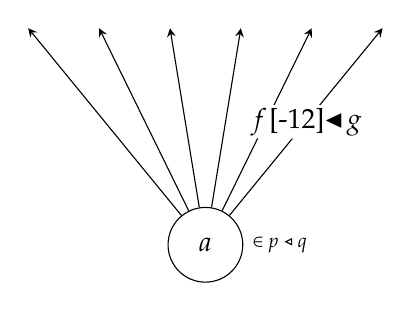
\begin{tikzpicture}
    \node [vertex,huger] (s) at (0, -12) {$a$};
    \coordinate (t11) at (-22.5,15.5) {};
    \coordinate (t12) at (-13.5,15.5) {};
    \coordinate (t13) at (-4.5,15.5) {};
    \coordinate (t21) at (4.5,15.5) {};
    \coordinate (t31) at (13.5,15.5) {};
    \coordinate (t32) at (22.5,15.5) {};
    \draw [edge] (s) -- (t11);
    \draw [edge] (s) -- (t12);
    \draw [edge] (s) -- (t13);
    \draw [edge] (s) -- (t21);
    \draw [edge] (s) -- (t31);
    \draw [edge] (s) -- node [label] {$f \subd g$} (t32);
    
    \node [annot] at (6, -12) {\rlap{$\posof p \sub q$}};
  \end{tikzpicture}
\end{center}
\vspace{1em}

We denote such a direction from such a position in a substitution
product by $f \subd g$. Accordingly, $\idsubd$ will denote the unique
direction from the unique position in the unit for substitution
$\idsub$ (a.k.a. the polynomial $y$).\footnote{Given directions $f$,
  $g$, and $h$ respectively belonging to polynomials $p$, $q$, and
  $r$, the directions of the form $(f \subd g)\subd h$ belonging to
  $(p \sub q) \sub r$ and the directions of the form
  $f \subd (g \subd h)$ belonging to $p \sub (q \sub r)$ are
  identified under the relevant monoidal coherence isomorphism. Hence
  brackets can be omitted.

  Similarly, for any direction $f$ belonging to a polynomial $p$, we
  have that $\idsubd \subd f$ and $f \subd \idsubd$ (respectively
  belonging to $\idsub \sub p$ and $p \sub \idsub$) are both
  canonically identified with $f$.}

\begin{prop}
  Polynomial comonoids are categories.
\end{prop}
\begin{proof}
  Let $c$ be a polynomial comonoid. Denote counit by $\varepsilon$
  and comultiplication by $\delta$.

\begin{center}
  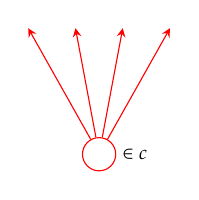
\begin{tikzpicture}
    \node [rcol,vertex,large] (s) at (0, -8) {};
    \coordinate (t1) at (-9,8) {};
    \coordinate (t2) at (-3,8) {};
    \coordinate (t3) at (3,8) {};
    \coordinate (t4) at (9,8) {};
    \draw [rcol,edge] (s) -- (t1);
    \draw [rcol,edge] (s) -- (t2);
    \draw [rcol,edge] (s) -- (t3);
    \draw [rcol,edge] (s) -- (t4);
    \node [annot] at (3, -8) {\rlap{$\posof c$}};
  \end{tikzpicture}
  \hspace{-.75em}
  $\underset{\varepsilon}{\transformto}$
  \begin{tikzpicture}
    \coordinate (s) at (0, -9.5) {};
    \coordinate (t1) at (-9,8) {};
    \coordinate (t2) at (-3,8) {};
    \coordinate (t3) at (3,8) {};
    \coordinate (t4) at (9,8) {};
    \draw [dash] (s) -- (t1);
    \draw [edge] (s) -- node [label] {\scriptsize$\idsubd$} (t2);
    \draw [dash] (s) -- (t3);
    \draw [dash] (s) -- (t4);
  \end{tikzpicture}
  \quad\qquad
  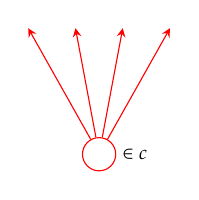
\begin{tikzpicture}
    \node [rcol,vertex,large] (s) at (0, -8) {};
    \coordinate (t1) at (-9,8) {};
    \coordinate (t2) at (-3,8) {};
    \coordinate (t3) at (3,8) {};
    \coordinate (t4) at (9,8) {};
    \draw [rcol,edge] (s) -- (t1);
    \draw [rcol,edge] (s) -- (t2);
    \draw [rcol,edge] (s) -- (t3);
    \draw [rcol,edge] (s) -- (t4);
    \node [annot] at (3, -8) {\rlap{$\posof c$}};
  \end{tikzpicture}
  \hspace{-.75em}
  $\underset{\delta}{\transformto}$
  \hspace{.5em}
  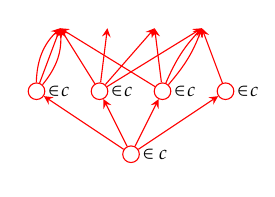
\begin{tikzpicture}
    \node [rcol,vertex] (s) at (0, -8) {};
    \coordinate (t1) at (-9,8) {};
    \coordinate (t2) at (-3,8) {};
    \coordinate (t3) at (3,8) {};
    \coordinate (t4) at (9,8) {};
    \node [rcol,vertex] (m1) at (-12,0) {};
    \node [rcol,vertex] (m2) at (-4,0) {};
    \node [rcol,vertex] (m3) at (4,0) {};
    \node [rcol,vertex] (m4) at (12,0) {};
    \draw [rcol,edge] (s) -- (m1);
    \draw [rcol,edge] (s) -- (m2);
    \draw [rcol,edge] (s) -- (m3);
    \draw [rcol,edge] (s) -- (m4);
    
    \draw [rcol,edge] (m1) -- (t1);
    \draw [rcol,edge,bend left=22] (m1) to (t1);
    \draw [rcol,edge,bend right=22] (m1) to (t1);
    
    \draw [rcol,edge] (m2) -- (t1);
    \draw [rcol,edge] (m2) -- (t2);
    \draw [rcol,edge] (m2) -- (t3);
    \draw [rcol,edge] (m2) -- (t4);
    
    \draw [rcol,edge] (m3) -- (t1);
    \draw [rcol,edge] (m3) -- (t3);
    \draw [rcol,edge,bend left=10] (m3) to (t4);
    \draw [rcol,edge,bend right=10] (m3) to (t4);
    
    \draw [rcol,edge] (m4) -- (t4);
    
    \node [annot] at (1.5, -8) {\rlap{$\posof c$}};
    
    \node [annot] at (-10.5, 0) {\rlap{$\posof\!c$}};
    \node [annot] at (-2.5, 0) {\rlap{$\posof\!c$}};
    \node [annot] at (5.5, 0) {\rlap{$\posof\!c$}};
    \node [annot] at (13.5, 0) {\rlap{$\posof\!c$}};
  \end{tikzpicture}
\end{center}

Observe first that the right unit law forces $(\posmap{\delta}(a))_\base = a$
for all $a \in \pos{c}$.

\begin{center}
  \begin{tikzpicture}
    \coordinate (s) at (0, -8) {};
    \coordinate (t1) at (-9,8) {};
    \coordinate (t2) at (-3,8) {};
    \coordinate (t3) at (3,8) {};
    \coordinate (t4) at (9,8) {};
    \node [rcol,vertex,transparent] (m1) at (-12,0) {};
    \node [rcol,vertex] (m2) at (-4,0) {};
    \node [rcol,vertex,transparent] (m3) at (4,0) {};
    \node [rcol,vertex,transparent] (m4) at (12,0) {};
    \draw [dash] (s) -- (m1);
    \draw [edge] (s) -- (m2);
    \draw [dash] (s) -- (m3);
    \draw [dash] (s) -- (m4);
    
    \draw [rcol,edge,transparent] (m1) -- (t1);
    \draw [rcol,edge,bend left=22,transparent] (m1) to (t1);
    \draw [rcol,edge,bend right=22,transparent] (m1) to (t1);
    
    \draw [rcol,edge] (m2) -- (t1);
    \draw [rcol,edge] (m2) -- (t2);
    \draw [rcol,edge] (m2) -- (t3);
    \draw [rcol,edge] (m2) -- (t4);
    
    \draw [rcol,edge,transparent] (m3) -- (t1);
    \draw [rcol,edge,transparent] (m3) -- (t3);
    \draw [rcol,edge,bend left=10,transparent] (m3) to (t4);
    \draw [rcol,edge,bend right=10,transparent] (m3) to (t4);
    
    \draw [rcol,edge,transparent] (m4) -- (t4);
    
    \node at (0, -13) {$(\varepsilon \sub \id_c) \circ \delta$};
  \end{tikzpicture}
  \quad
  $\canoniso$
  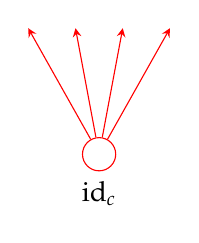
\begin{tikzpicture}
    \node [rcol,vertex,large] (s) at (0, -8) {};
    \coordinate (t1) at (-9,8) {};
    \coordinate (t2) at (-3,8) {};
    \coordinate (t3) at (3,8) {};
    \coordinate (t4) at (9,8) {};
    \draw [rcol,edge] (s) -- (t1);
    \draw [rcol,edge] (s) -- (t2);
    \draw [rcol,edge] (s) -- (t3);
    \draw [rcol,edge] (s) -- (t4);
    
    \node at (0, -13) {$\id_c$};
  \end{tikzpicture}
  $\canoniso$
  \quad
  \begin{tikzpicture}
    \node [rcol,vertex] (s) at (0, -8) {};
    \coordinate (t1) at (-9,8) {};
    \coordinate (t2) at (-3,8) {};
    \coordinate (t3) at (3,8) {};
    \coordinate (t4) at (9,8) {};
    \coordinate (m1) at (-12,0) {};
    \coordinate (m2) at (-4,0) {};
    \coordinate (m3) at (4,0) {};
    \coordinate (m4) at (12,0) {};
    \draw [rcol,edge] (s) -- (m1);
    \draw [rcol,edge] (s) -- (m2);
    \draw [rcol,edge] (s) -- (m3);
    \draw [rcol,edge] (s) -- (m4);
    
    \draw [edge] (m1) -- (t1);
    \draw [dash,bend left=22] (m1) to (t1);
    \draw [dash,bend right=22] (m1) to (t1);
    
    \draw [dash] (m2) -- (t1);
    \draw [edge] (m2) -- (t2);
    \draw [dash] (m2) -- (t3);
    \draw [dash] (m2) -- (t4);
    
    \draw [dash] (m3) -- (t1);
    \draw [edge] (m3) -- (t3);
    \draw [dash,bend left=10] (m3) to (t4);
    \draw [dash,bend right=10] (m3) to (t4);
    
    \draw [edge] (m4) -- (t4);
    
    \node at (0, -13) {$(\id_c \sub \varepsilon) \circ \delta$};
  \end{tikzpicture}
\end{center}
Therefore the expression $(\posmap{\delta}(a))_f$ for $f \in c[a]$ has a
well-defined meaning.

We gather the data of a category $\mathcal{C}$.
\begin{itemize}
\item The set of objects $\Ob(\mathcal{C})$ is $\pos{c}$, i.e., the set
  of positions in $c$.
\item The set of arrows $\Arr(\mathcal{C})$ is
  $\sum_{a \in \pos{c}}c[a]$, i.e., the set of all directions in $c$.
\item The source map $s$ sends each $f \in c[a]$ to $a$. (Hence the
  polynomial $c$ is described by the bundle
  $\Arr(\mathcal{C}) \bundle{s} \Ob(\mathcal{C})$.)
\item The target map $t$ sends each $f \in c[a]$ to $(\posmap{\delta}(a))_f$.
\item The identity map $e$ sends each $a \in \pos{c}$ to
  $\varepsilon^\sharp(a, \idsubd)$.
\item The composition map $m$ sends each pair of compatible
  arrows ${f \in c[a]}, {g \in c[t(f)]}$ to $\delta^\sharp(a, f \subd g)$.
\end{itemize}

Now we verify these data satisfy the laws of a category.
\begin{itemize}
\item The law $s(e(a)) = a$ is true by construction; $e(a)$ is a
  direction from the position $a$.
\item The law $t(e(a)) = a$ is forced to hold by the comonoid left
  unit law, which identifies  with .
\item The law $s(m(f, g)) = s(f)$ is true by construction; $m(f, g)$
  is a direction from the position $s(f)$.
\item The law $t(m(f, g)) = t(g)$ .
\item The left unit law $m(e(s(f)), f) = f$ is directly expressed by
  the comonoid left unit law.
\item The right unit law $m(f, e(t(f))) = f$ is directly expressed by
  the comonoid right unit law.
\item The associativity law $m(m(f, g) h) = m(f, m(g, h))$ is directly
  expressed by the comonoid associativity law.
\end{itemize}

\begin{center}
  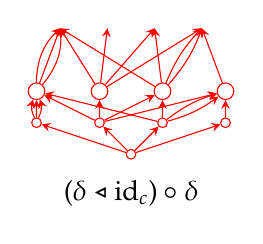
\begin{tikzpicture}
      \node [rcol,vertex,small] (s) at (0, -8) {};
      \coordinate (t1) at (-9,8) {};
      \coordinate (t2) at (-3,8) {};
      \coordinate (t3) at (3,8) {};
      \coordinate (t4) at (9,8) {};
      
      \node [rcol,vertex,small] (m1_) at (-12,-4) {};
      \node [rcol,vertex,small] (m2_) at (-4,-4) {};
      \node [rcol,vertex,small] (m3_) at (4,-4) {};
      \node [rcol,vertex,small] (m4_) at (12,-4) {};
      \draw [rcol,edge] (s) -- (m1_);
      \draw [rcol,edge] (s) -- (m2_);
      \draw [rcol,edge] (s) -- (m3_);
      \draw [rcol,edge] (s) -- (m4_);
      
      \node [rcol,vertex] (m1) at (-12,0) {};
      \node [rcol,vertex] (m2) at (-4,0) {};
      \node [rcol,vertex] (m3) at (4,0) {};
      \node [rcol,vertex] (m4) at (12,0) {};
      
      \draw [rcol,edge] (m1_) -- (m1);
      \draw [rcol,edge,bend left=22] (m1_) to (m1);
      \draw [rcol,edge,bend right=22] (m1_) to (m1);
      
      \draw [rcol,edge] (m2_) -- (m1);
      \draw [rcol,edge] (m2_) -- (m2);
      \draw [rcol,edge] (m2_) -- (m3);
      \draw [rcol,edge] (m2_) -- (m4);
      
      \draw [rcol,edge] (m3_) -- (m1);
      \draw [rcol,edge] (m3_) -- (m3);
      \draw [rcol,edge,bend left=10] (m3_) to (m4);
      \draw [rcol,edge,bend right=10] (m3_) to (m4);
      
      \draw [rcol,edge] (m4_) -- (m4);

      
      \draw [rcol,edge] (m1) -- (t1);
      \draw [rcol,edge,bend left=22] (m1) to (t1);
      \draw [rcol,edge,bend right=22] (m1) to (t1);
      
      \draw [rcol,edge] (m2) -- (t1);
      \draw [rcol,edge] (m2) -- (t2);
      \draw [rcol,edge] (m2) -- (t3);
      \draw [rcol,edge] (m2) -- (t4);
      
      \draw [rcol,edge] (m3) -- (t1);
      \draw [rcol,edge] (m3) -- (t3);
      \draw [rcol,edge,bend left=10] (m3) to (t4);
      \draw [rcol,edge,bend right=10] (m3) to (t4);
      
      \draw [rcol,edge] (m4) -- (t4);
      
      \node at (0, -13) {$(\delta \sub \id_c) \circ \delta$};
  \end{tikzpicture}
  \quad
  $\canoniso$
  \quad
  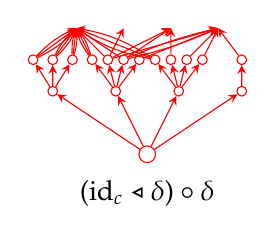
\begin{tikzpicture}
      \node [rcol,vertex] (s) at (0, -8) {};
      \coordinate (t1) at (-9,8) {};
      \coordinate (t2) at (-3,8) {};
      \coordinate (t3) at (3,8) {};
      \coordinate (t4) at (9,8) {};
      
      \node [rcol,vertex,small] (m1) at (-12,0) {};
      \node [rcol,vertex,small] (m2) at (-4,0) {};
      \node [rcol,vertex,small] (m3) at (4,0) {};
      \node [rcol,vertex,small] (m4) at (12,0) {};
      \draw [rcol,edge] (s) -- (m1);
      \draw [rcol,edge] (s) -- (m2);
      \draw [rcol,edge] (s) -- (m3);
      \draw [rcol,edge] (s) -- (m4);

      \node [rcol,vertex,small] (m11) at (-14.5,4) {};
      \node [rcol,vertex,small] (m12) at (-12,4) {};
      \node [rcol,vertex,small] (m13) at (-9.5,4) {};
      \node [rcol,vertex,small] (m21) at (-7,4) {};
      \node [rcol,vertex,small] (m22) at (-5,4) {};
      \node [rcol,vertex,small] (m23) at (-3,4) {};
      \node [rcol,vertex,small] (m24) at (-1,4) {};
      \node [rcol,vertex,small] (m31) at (1,4) {};
      \node [rcol,vertex,small] (m32) at (3,4) {};
      \node [rcol,vertex,small] (m33) at (5,4) {};
      \node [rcol,vertex,small] (m34) at (7,4) {};
      \node [rcol,vertex,small] (m41) at (12,4) {};
      
      \draw [rcol,edge] (m1) -- (m11);
      \draw [rcol,edge] (m1) -- (m12);
      \draw [rcol,edge] (m1) -- (m13);
      \draw [rcol,edge] (m2) -- (m21);
      \draw [rcol,edge] (m2) -- (m22);
      \draw [rcol,edge] (m2) -- (m23);
      \draw [rcol,edge] (m2) -- (m24);
      \draw [rcol,edge] (m3) -- (m31);
      \draw [rcol,edge] (m3) -- (m32);
      \draw [rcol,edge] (m3) -- (m33);
      \draw [rcol,edge] (m3) -- (m34);
      \draw [rcol,edge] (m4) -- (m41);

      
      \draw [rcol,edge] (m11) -- (t1);
      \draw [rcol,edge,bend left=11] (m11) to (t1);
      \draw [rcol,edge,bend right=11] (m11) to (t1);
      
      \draw [rcol,edge] (m12) -- (t1);
      \draw [rcol,edge,bend left=11] (m12) to (t1);
      \draw [rcol,edge,bend right=11] (m12) to (t1);
      
      \draw [rcol,edge] (m13) -- (t1);
      \draw [rcol,edge,bend left=11] (m13) to (t1);
      \draw [rcol,edge,bend right=11] (m13) to (t1);
      
      
      \draw [rcol,edge] (m21) -- (t1);
      \draw [rcol,edge,bend left=11] (m21) to (t1);
      \draw [rcol,edge,bend right=11] (m21) to (t1);
      
      \draw [rcol,edge] (m22) -- (t1);
      \draw [rcol,edge] (m22) -- (t2);
      \draw [rcol,edge] (m22) -- (t3);
      \draw [rcol,edge] (m22) -- (t4);
      
      \draw [rcol,edge] (m23) -- (t1);
      \draw [rcol,edge] (m23) -- (t3);
      \draw [rcol,edge,bend left=5] (m23) to (t4);
      \draw [rcol,edge,bend right=5] (m23) to (t4);
      
      \draw [rcol,edge] (m24) -- (t4);

      
      \draw [rcol,edge] (m31) -- (t1);
      \draw [rcol,edge,bend left=11] (m31) to (t1);
      \draw [rcol,edge,bend right=11] (m31) to (t1);
      
      \draw [rcol,edge] (m32) -- (t3);
      
      \draw [rcol,edge] (m33) -- (t4);
      
      \draw [rcol,edge] (m34) -- (t4);

      
      \draw [rcol,edge] (m41) -- (t4);
      
      \node at (0, -13) {$(\id_c \sub \delta) \circ \delta$};
  \end{tikzpicture}
\end{center}

Conversely, let $\mathcal{C}$ be a category. We immediately obtain the
bundle ${\Arr(\mathcal{C})\bundle{s}\Ob(\mathcal{C})}$. Let $c$ denote
the polynomial described by this bundle (the ``outfacing polynomial''
of $\mathcal{C}$); we exhibit a comonoid struture on $c$.c

Lastly, these translation processes between polynomial comonoids
and categories are inverse by construction.
\end{proof}

\begin{prop}
  A polynomial left comodule amounts to a copresheaf and a presheaf on
  that copresheaf's category of elements.
\end{prop}
\begin{proof}
  Let $c$ be a polynomial comonoid and let $m$ be a left comodule on
  $c$. Denote left comodule comultiplication by $\lambda$.

  \begin{center}
    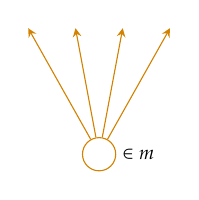
\begin{tikzpicture}
      \node [ycol,vertex,large] (s) at (0, -8) {};
      \coordinate (t1) at (-9,8) {};
      \coordinate (t2) at (-3,8) {};
      \coordinate (t3) at (3,8) {};
      \coordinate (t4) at (9,8) {};
      \draw [ycol,edge] (s) -- (t1);
      \draw [ycol,edge] (s) -- (t2);
      \draw [ycol,edge] (s) -- (t3);
      \draw [ycol,edge] (s) -- (t4);
      \node [annot] at (3, -8) {\rlap{$\posof m$}};
    \end{tikzpicture}
    \hspace{-.75em}
    $\underset{\lambda}{\transformto}$
    \hspace{.5em}
    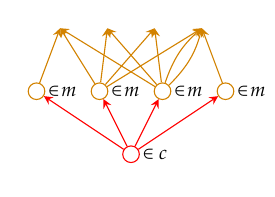
\begin{tikzpicture}
      \node [rcol,vertex] (s) at (0, -8) {};
      \coordinate (t1) at (-9,8) {};
      \coordinate (t2) at (-3,8) {};
      \coordinate (t3) at (3,8) {};
      \coordinate (t4) at (9,8) {};
      \node [ycol,vertex] (m1) at (-12,0) {};
      \node [ycol,vertex] (m2) at (-4,0) {};
      \node [ycol,vertex] (m3) at (4,0) {};
      \node [ycol,vertex] (m4) at (12,0) {};
      \draw [rcol,edge] (s) -- (m1);
      \draw [rcol,edge] (s) -- (m2);
      \draw [rcol,edge] (s) -- (m3);
      \draw [rcol,edge] (s) -- (m4);
      
      \draw [ycol,edge] (m1) -- (t1);
      
      \draw [ycol,edge] (m2) -- (t1);
      \draw [ycol,edge] (m2) -- (t2);
      \draw [ycol,edge] (m2) -- (t3);
      \draw [ycol,edge] (m2) -- (t4);
      
      \draw [ycol,edge] (m3) -- (t1);
      \draw [ycol,edge] (m3) -- (t2);
      \draw [ycol,edge] (m3) -- (t3);
      \draw [ycol,edge,bend left=15] (m3) to (t4);
      \draw [ycol,edge,bend right=15] (m3) to (t4);
      
      \draw [ycol,edge] (m4) -- (t4);
      
      \node [annot] at (1.5, -8) {\rlap{$\posof c$}};
      
      \node [annot] at (-10.5, 0) {\rlap{$\posof\!m$}};
      \node [annot] at (-2.5, 0) {\rlap{$\posof\!m$}};
      \node [annot] at (5.5, 0) {\rlap{$\posof\!m$}};
      \node [annot] at (13.5, 0) {\rlap{$\posof\!m$}};
    \end{tikzpicture}
  \end{center}

\end{proof}

\begin{prop}
  A polynomial right comodule amounts to a set of copresheaves.
\end{prop}
\begin{proof}
  Let $d$ be a polynomial comonoid and let $m$ be a right comodule on
  $d$. Denote right comodule comultiplication by $\rho$.

\begin{center}
  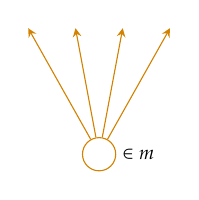
\begin{tikzpicture}
    \node [ycol,vertex,large] (s) at (0, -8) {};
    \coordinate (t1) at (-9,8) {};
    \coordinate (t2) at (-3,8) {};
    \coordinate (t3) at (3,8) {};
    \coordinate (t4) at (9,8) {};
    \draw [ycol,edge] (s) -- (t1);
    \draw [ycol,edge] (s) -- (t2);
    \draw [ycol,edge] (s) -- (t3);
    \draw [ycol,edge] (s) -- (t4);
    \node [annot] at (3, -8) {\rlap{$\posof m$}};
  \end{tikzpicture}
  \hspace{-.75em}
  $\underset{\rho}{\transformto}$
  \hspace{.5em}
  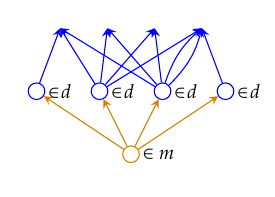
\begin{tikzpicture}
    \node [ycol,vertex] (s) at (0, -8) {};
    \coordinate (t1) at (-9,8) {};
    \coordinate (t2) at (-3,8) {};
    \coordinate (t3) at (3,8) {};
    \coordinate (t4) at (9,8) {};
    \node [bcol,vertex] (m1) at (-12,0) {};
    \node [bcol,vertex] (m2) at (-4,0) {};
    \node [bcol,vertex] (m3) at (4,0) {};
    \node [bcol,vertex] (m4) at (12,0) {};
    \draw [ycol,edge] (s) -- (m1);
    \draw [ycol,edge] (s) -- (m2);
    \draw [ycol,edge] (s) -- (m3);
    \draw [ycol,edge] (s) -- (m4);
    
    \draw [bcol,edge] (m1) -- (t1);
    
    \draw [bcol,edge] (m2) -- (t1);
    \draw [bcol,edge] (m2) -- (t2);
    \draw [bcol,edge] (m2) -- (t3);
    \draw [bcol,edge] (m2) -- (t4);
    
    \draw [bcol,edge] (m3) -- (t1);
    \draw [bcol,edge] (m3) -- (t2);
    \draw [bcol,edge] (m3) -- (t3);
    \draw [bcol,edge,bend left=15] (m3) to (t4);
    \draw [bcol,edge,bend right=15] (m3) to (t4);
    
    \draw [bcol,edge] (m4) -- (t4);
    
    \node [annot] at (1.5, -8) {\rlap{$\posof m$}};
    
    \node [annot] at (-10.5, 0) {\rlap{$\posof\!d$}};
    \node [annot] at (-2.5, 0) {\rlap{$\posof\!d$}};
    \node [annot] at (5.5, 0) {\rlap{$\posof\!d$}};
    \node [annot] at (13.5, 0) {\rlap{$\posof\!d$}};
  \end{tikzpicture}
\end{center}

\end{proof}

\begin{prop}
  Polynomial bicomodules are prafunctors.
\end{prop}
\begin{proof}
  
\end{proof}

\begin{prop}
  Maps between bicomodules are natural transformations between prafunctors.
\end{prop}
\begin{proof}
  
\end{proof}

\begin{prop}
  Composition of bicomodules is composition of prafunctors.
\end{prop}
\begin{proof}
  Recall bicomodules from $d$ to $0$ are copresheaves on $d$ (and maps
  between such bicomodules are copresheaf maps). Hence each bicomodule
  $m$ from $c$ to $d$ induces a functor $F_m$ from $d$-copresheaves to
  $c$-copresheaves by precomposition. Accordingly, we have
  $F_{m \sub_d n} \cong F_m \circ F_n$ (for bicomodules $m$
  from $c$ to $d$ and $n$ from $d$ to $e$).
  
  We show that the prafunctor corresponding to the bimodule $m$ is $F_m$. 
\end{proof}

\end{document}